\documentclass[10pt,journal,cspaper,compsoc]{IEEEtran}
\usepackage[]{lipsum}
\usepackage{cite}
\usepackage{amsmath,amssymb}
\usepackage{algorithm}
\usepackage{algorithmic}
\usepackage{multirow}
\usepackage{mathtools}

\usepackage[aboveskip=8pt]{caption}

\usepackage[dvips]{graphicx}
\DeclareGraphicsExtensions{.pdf}
\usepackage[american]{babel}

\usepackage{tabularx}


\usepackage{url}
\usepackage{cvpr}
\usepackage{multicol}

\usepackage{stfloats}
\usepackage{fixltx2e}
\usepackage{subfig}
\usepackage[bookmarks=false,colorlinks=true,linkcolor=black,citecolor=black,filecolor=black,urlcolor=black]{hyperref}

\newcommand{\cb}[1]{\textbf{#1}}
\newcommand{\ct}[1]{\fontsize{7pt}{1pt}\selectfont{#1}}
\newcommand{\tn}[1]{\footnotesize{#1}}
\newcommand{\code}[1]{\texttt{#1}}
\newcolumntype{x}{>\small c}


\def\cls{\mathit{cls}}
\def\reg{\mathit{reg}}

%\renewcommand{\floatpagefraction}{0.1}
%\renewcommand{\bottomfraction}{0.1}
%\renewcommand{\topfraction}{1}
%\renewcommand{\textfraction}{0.0}
\renewcommand{\dbltopfraction}{1.0}
\renewcommand{\dblfloatpagefraction}{0.0}

\newcommand{\tabincell}[2]{\begin{tabular}{@{}#1@{}}#2\end{tabular}}

\DeclarePairedDelimiter\ceil{\lceil}{\rceil}
\DeclarePairedDelimiter\floor{\lfloor}{\rfloor}


\title{Mine-RCNN}

\begin{document}


    \author{Loi~Dario (1940849),
        Marincione~Davide (1927757),
        Barda~Benjamin (1805213)% <-this % stops a space
    }
%\IEEEcompsocitemizethanks{
%\IEEEcompsocthanksitem S. Ren is with University of Science and Technology of China, Hefei, China. This work was done when S. Ren was an intern at Microsoft Research. Email: sqren@mail.ustc.edu.cn
%\IEEEcompsocthanksitem K.~He and J.~Sun are with Visual Computing Group, Microsoft Research. E-mail: \{kahe,jiansun\}@microsoft.com
%\IEEEcompsocthanksitem R.~Girshick is with Facebook AI Research. The majority of this work was done when R. Girshick was with Microsoft Research. E-mail: rbg@fb.com}
%}

\IEEEcompsoctitleabstractindextext{%
\begin{abstract}
    Real time object detection has recently been made possible due to steady state-of-the-art advancements in the field \cite{arxiv:FastRCNN,arxiv:FasterRCNN}, these methods propose the use of a Region Proposal Network to 
    identify Regions of Interest (RoIs) in the image and correctly classify them, we aim to reproduce the architecture proposed by \cite{arxiv:FasterRCNN} applied to a novel environment, that of the
    popular sandbox Minecraft, both for the ease-of-collection of the required data and for a number of graphical properties possesed by the game that make such a complex problem more approachable in terms 
    of computational resources, moreover, due to the novelty of the environment, we also train the entirety of the network from the ground up, having no pre-trained backbone at our disposal.
\end{abstract}

%State-of-the-art object detection networks depend on region proposal algorithms to hypothesize object locations. Advances like SPPnet and Fast R-CNN have reduced the running time of these detection networks, exposing region proposal computation as a bottleneck. In this work, we introduce a Region Proposal Network (RPN) that shares full-image convolutional features with the detection network, thus enabling nearly cost-free region proposals. An RPN is a fully convolutional network that simultaneously predicts object bounds and objectness scores at each position. The RPN is trained end-to-end to generate high-quality region proposals, which are used by Fast R-CNN for detection. We further merge RPN and Fast R-CNN into a single network by sharing their convolutional features---using the recently popular terminology of neural networks with 'attention' mechanisms, the RPN component tells the unified network where to look. For the very deep VGG-16 model, our detection system has a frame rate of 5fps (including all steps) on a GPU, while achieving state-of-the-art object detection accuracy on PASCAL VOC 2007, 2012, and MS COCO datasets with only 300 proposals per image. In ILSVRC and COCO 2015 competitions, Faster R-CNN and RPN are the foundations of the 1st-place winning entries in several tracks. Code has been made publicly available.

% Note that keywords are not normally used for peer review papers.
\begin{IEEEkeywords}
 Object Detection, Convolutional Neural Network, Sandbox, Region Proposal, Real Time Detection
\end{IEEEkeywords}}

\maketitle
\IEEEpeerreviewmaketitle
    
\begin{figure*}[tb]
    
    \centering
    \subfloat[Our Backbone]{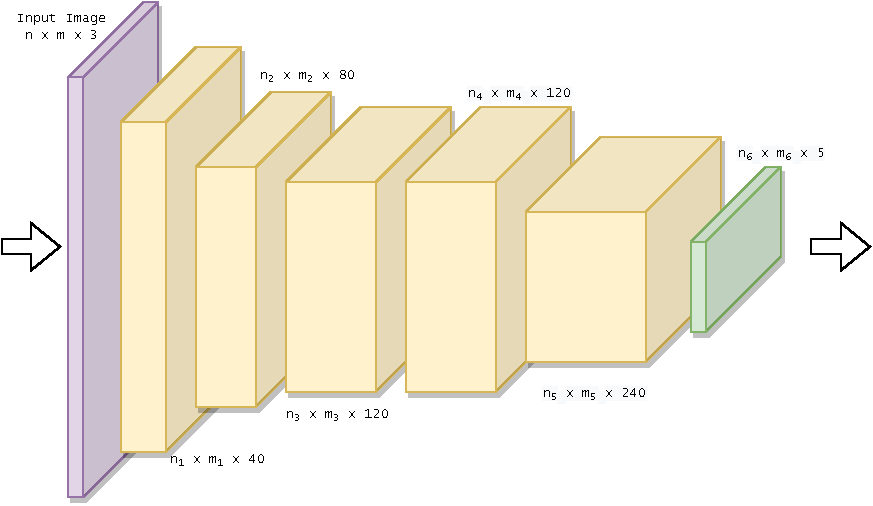
\includegraphics[width=0.45\textwidth]{images/backbone.pdf}} \hfill
    \subfloat[Our Network]{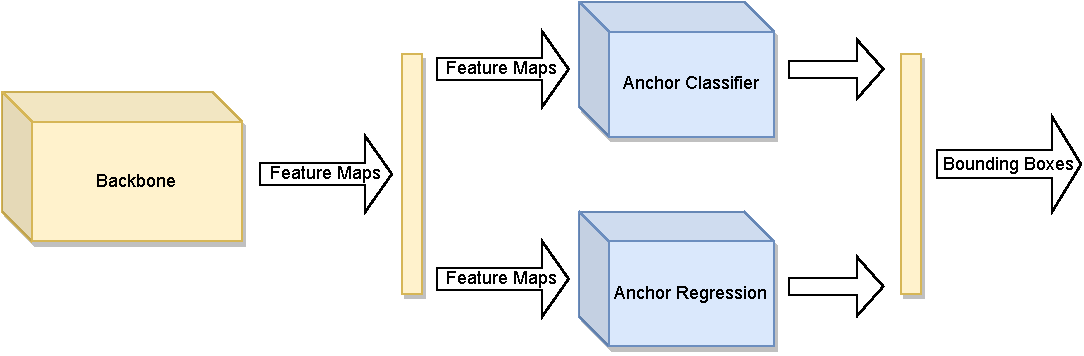
\includegraphics[width=0.45\textwidth]{images/network.pdf}}
    \caption{Our FCNN backbone (a) employs a series of convolutions to obtain a feature map to pass to 
    the rest of the network as displayed in (b), the feature maps from our Backbone are first pre-processed
    by a sliding-window approach that spreads our anchors over the image, this is then passed to a twin neural
    network, one part of the network performs classification, determining if each bounding box is containing an
    object or not, the other part performs regression on our bounding box in order to make it better fit an eventual
    target object.}
    \label{fig:network}
\end{figure*}


\begin{figure}[tb]
    \centering
    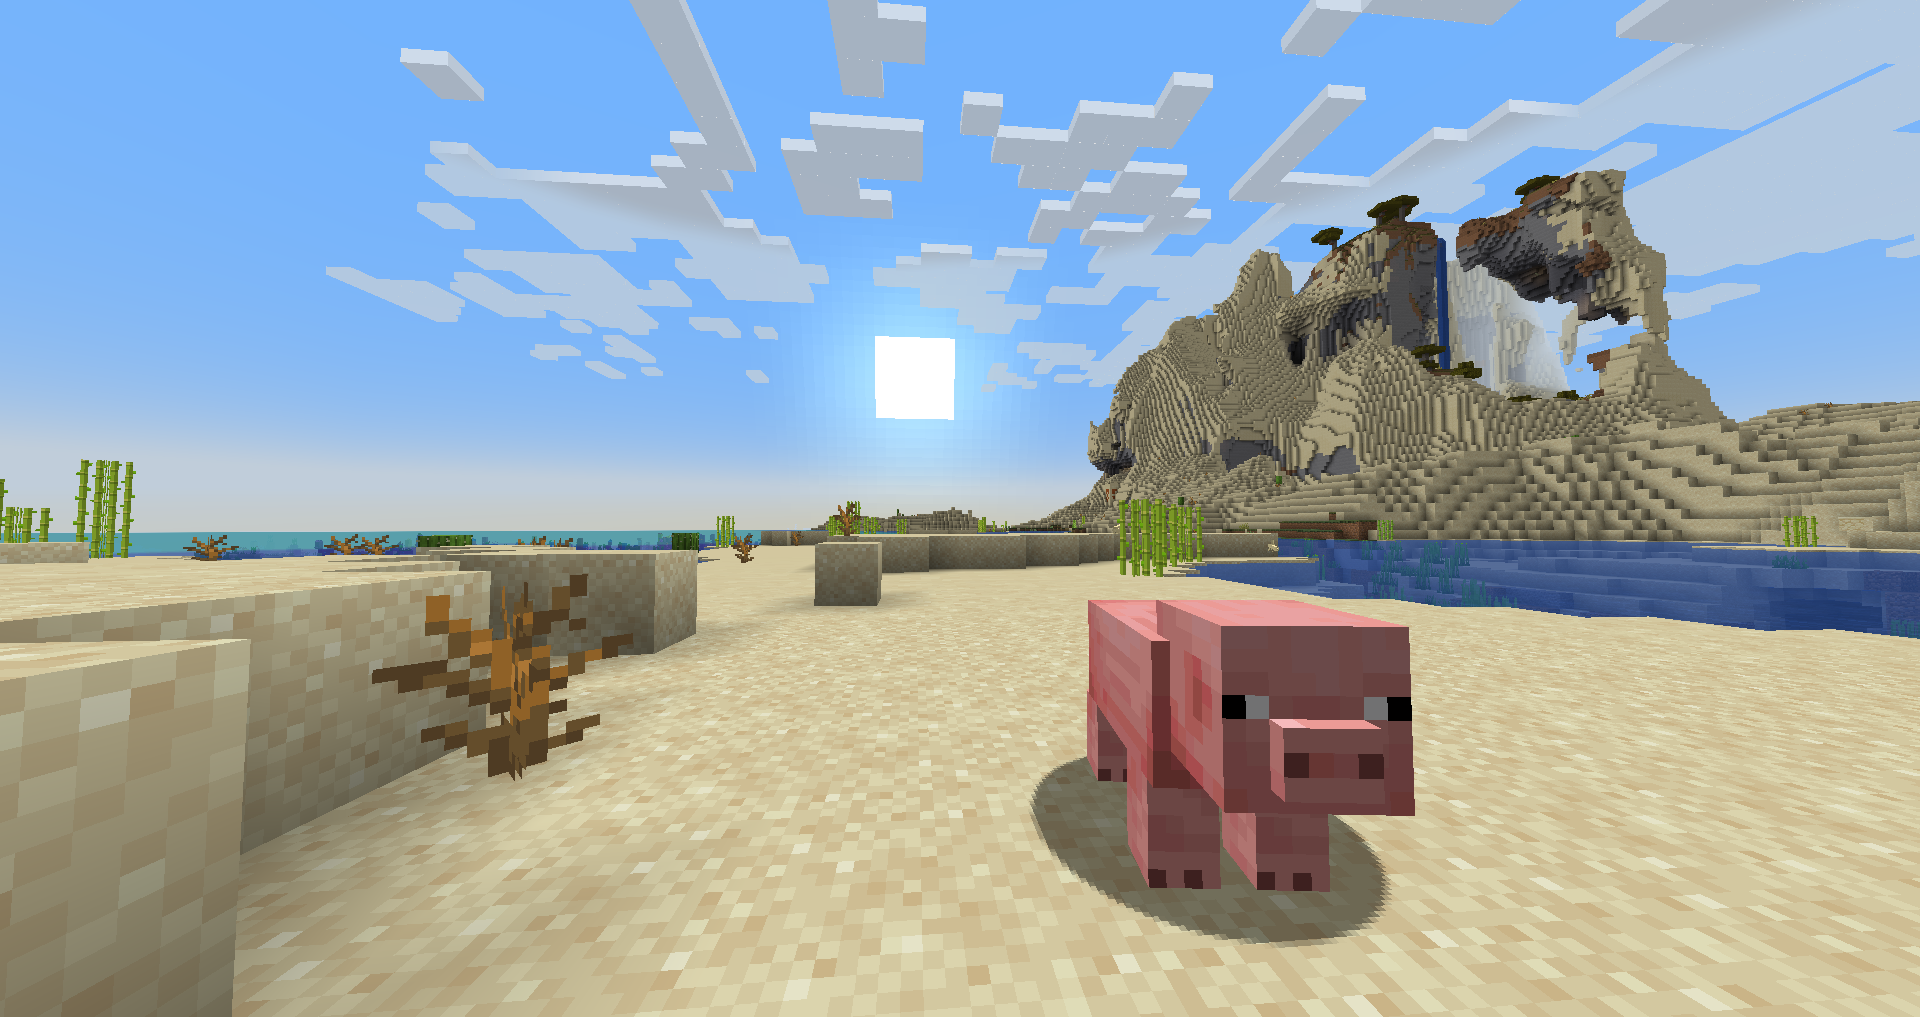
\includegraphics[width=0.44\textwidth]{images/pig.png}
    \caption{A Screenshot of the world of Minecraft, note the simplistic graphics and the absence of Bloom (except the illusion thereof provided by the 
    skybox) even though we are staring directly at the sun, note also the presence of a \emph{pig}, one of the entities that we are going to detect 
    in our model.}
    \label{fig:piggy}
\end{figure}

    \section{Introduction}
    Traditional visual recognition algorithms employ the use of algorithms such as SIFT 
    or SURF\cite{Lowe:SIFT,Bay:SURF}, to extract a feature descriptor from key points 
    in the image, a set of sample images is therefore processed in order to obtain descriptors 
    for each class, inference is then performed by extracting the descriptor from the input image 
    and then comparing it with our samples, using a distance criterion to select the closest class.

    While these traditional methods are mostly invariant to scale and translations, issues such as 
    variability in the brightness or rotation of the target object are problematic, moreover, the 
    computational cost of extracting features is prohibitively high, effectively preventing the possibility
    of deploying the model in a real-time context.

    \paragraph*{Our Approach}
    One way to reduce the cost in performance while gaining a higher expressive capacity for our model is to employ
    modern Deep Learning techniques to build our detector, our aim is therefore to 
    design a scaled-back version of \cite{arxiv:FasterRCNN}, stopping ourselves at the classification stage,
    the reason for this will be further clarified in the rest of the paper, our architecture\footnote{see 
    Figure \ref{fig:network} for a diagram
    of our architecture} is composed of a FCNN\cite{Chen:FCNN,Simonyan:VCC16} Backbone, this is to keep the number 
    of parameters as low as possible as well as allow the initial layer of our architecture to be applicable to images 
    of any resolution, our Convolutional Backbone must be trained from the ground up in the task of simply classifying 
    the classes that we intend to detect, the classifying layer is then removed from the model and we're then
    left with its feature map output which we then pre-process by \emph{splashing} anchors through a sliding window 
    approach.

        

    After this, both feature maps and anchors are then passed to our region proposal layers, which in turn is composed 
    of a twin ensemble of Neural Networks that perform Regression and Classification on the bounding boxes, the outcome is a set of 
    \emph{positive} and \emph{negative} bounding boxes, the boxes that are classified as positive 
    go through NMS\cite{Neubeck:NMS} using Intersection over Union (IoU) \cite{Rezatofighi:IoU} as a metric for suppression
    in order to reduce the amount of individual boxes that classify the same object.

    
    \paragraph*{Our Environment}
    In order to keep our project in the realms of feasibility, especially considering the constraints imposed on our team in the 
    realms of time and processing capabilities of our hardware, we chose to detect objects in a virtual environment, this is because 
    the possibility of having complete control over the environment allows us to artificially create scenarios from which we can gather 
    samples of a large quantity, for this reason, we chose the popular sandbox game Minecraft \cite{Mojang-Minecraft}, other than 
    the advantage of control over the environment, the game is well known for it's simplistic approach to Voxel Graphics, rendering 
    the world as a set of blocks of cubic shape, the game also possesses a simplistic lightning model that simply shifts the brightness
    of blocks' textures when in the vicinity of a light source, thus being void of effects such as bloom, specular components on objects,
    reflections and other complex techniques that introduce sources of unexpected noise or variability in our samples, this, in turn, 
    allows our model to work in a context that, while still posing a significant challenge, is of suitable difficulty to the scope of 
    this project.



 \section{Method}   
    \subsection{The Dataset}
    We first started by building a dataset. We recorded one-minutes long videos of Minecraft using commercial screen capture software, we then loaded those shorts into python using the OpenCV library, we then arbitrarily sampled frames from the videos at a rate of 1 frame-per-second, as we assume this rate to be sufficient to provide a good number of samples while also ensuring a good variability in-between our frames. 

    We downsampled the images from 1080p to 240p to reduce the size of the dataset in order to both be able to share it with ease and load it in GPU memory even when the hardware at hand is a common, low capacity commercial card. By convention, we decided it would be better for the image to be resized at a 1:1 aspect ratio, in order to try and preserve the same amount of information, we decided to choose a size that would keep the area almost constant:

    \begin{equation}\label{eq:area}
        \begin{aligned}
            A &= w * h \\
            &= 240 \cdot 426\\ 
            &= 102'240\\
            l &= \floor*{\sqrt{w * h}} = 319\\
            l^2 &= 101'761 \approx A\\
        \end{aligned}
    \end{equation} 
    
    At this time we opted to limit ourselves to only five classes for: Zombies, Creepers, Pigs, Sheep, Nothing.
    The first iteration of the Dataset was comprised of images that contained multiple classes in the same scene, this was because our initial idea was to diverge from the implementation described in \cite{arxiv:FasterRCNN} and implement a particular form of loss called \emph{Triplet Loss}\cite{Chechik:Triplet}, this proved problematic since when training the backbone we were presented with problems of exploding gradients and general failure of the network to converge, this idea was then discarded on the ground of practicality and the focus of the 
    project shifted back to training a traditional classifier that uses Cross-Entropy as a loss function, for this reason the Dataset was also re-done from the ground up to only have a single object in the frame at a time,
    The next step consisted in manually labelling each one of the sampled frames. We developed a simple but effective tool that allowed us to draw bounding boxes\footnote{BBoxes for brevity.} and assign to each one of them a label corresponding to one of the classes mentioned above. During this process we pruned the images that we considered
    unfit to be part of the dataset (e.g. frames inside the game menu or outside of the game). After standardizing the coordinates of BBoxes we saved them into JSONs files, after having our JSONS files ready we group them into a single .dtst\footnote{Our own extension, stands for \emph{dataset}.} file for better integration with \code{PyTorch}.
    
    \paragraph*{Data Augmentation}
    Due to the reduced amount of resources, manpower and time available to us when compared to professional teams, we considered \emph{a priori} the size of our dataset to be small\footnote{funnily enough, the final result of $\approx4000$ images is quite a sizeable dataset considering the complexity of our environment.}, and therefore 
    prone to overfitting, we pre-emptively took approaches in order to stave off overfitting, one such approach was the applying of a set of random transformations on each input image 
    in order to increase the variability and artificially inflate the size of our dataset, these were, for the purpose of classification:
    \begin{enumerate}
        \item Reflecting the image horizontally with $p = 0.5$
        \item Scaling the image's brightness, contrast and saturation 
        with factors $(b, c, s)$ chosen uniformly over 
        the intervals: $b \in [0.60, 1.40], c \in [0.95, 1.05], s \in [0.99, 1.01]$
        \item Randomly downscaling the sharpness of the image with a factor $k_1 = 1.25, p = 0.2$
        \item Randomly upscaling the sharpness of the image with a factor $k_1 = 0.75, p = 0.2$
        \item Applying a random rotation 
        in the interval $\theta \in [-15^{\circ}, 15^{\circ}]$
    \end{enumerate}
    Whereas, during the training of the full network, only the color-related transformations were kept 
    due to the others requiring non-trivial customizations in order to also be correctly applied to each 
    image's set of ground-truth bounding boxes. 
    
    \subsection{The Models}
    Our architecture is divided into two main modules: The Backbone, which we decided to call the "Ziggurat" (ZG), and the Region Proposal Network (RPN).

    \paragraph*{The Backbone: Ziggurat}
    The ZG is a Fully convolutional neural network consisting of 6 layers as described in table \ref{tab:Table 1}, the sixth layer of which will be dropped after the pre-training phase. 
    The purpose of this network is to extract feature maps from the input image for the RPN that follows,
    It is important then to pre-train this network so that it learns the general embedding in order 
    to reduce the complexity of training the RPN. 
    We decided to add dropout layers as they provide a useful guard against overfitting \cite{Srivastava:Dropout}, and, again, considering the dimensions of our dataset we decided to add it to each layer except the last one. For the activation function we decided to use MISH opposed to ReLU used in the original Faster-RCNN as it is already 
    widely accepted as superior in terms of stability and accuracy, due to the smoothness of it's first derivative and the lack of vanishing gradient problems that plague ReLU, The weights were initialized using the Kaiming method as proposed by \cite{arxiv:Kaiming}.
    \begin{table*}[htb]
        \centering
		\caption{ZG}
		\label{tab:Table 1}
		\begin{tabularx}{.9\paperwidth}{l | c | c | c | c |  l}  
			\textbf{Layer} & \textbf{Kernel size} & \textbf{IN/OUT channels} & \textbf{padding} & \textbf{stride} & \textbf{Layer Structure}\\
			\hline 
			& & & & & \\
			1 & 7x7 & 3 / 40 & replicate(1) & 2 & BATCHNORM(3) + CONV + MISH + DROPOUT(.2) + BATCHNORM(40) \\
			2 & 7x7 & 40 / 80 & replicate(1) & 2 & CONV + MISH + DROPOUT(.2) + BATCHNORM(80) \\
			3 & 3x3 & 80 / 120 & replicate(1) & 2 & CONV + MISH + DROPOUT(.2) + BATCHNORM(80) \\ 
			4 & 3x3 & 120/120 & None & 1 & CONV + MISH + DROPOUT(.2) + BATCHNORM(120)  \\
			5 & 3x3 & 120/240 & replicate(1) & 2 & CONV + MISH + DROPOUT(.2) + BATCHNORM(240) \\
			& & & & & \\
			\hline
			& & & & & \\
			6 & 1x1 & 240/5 & None & 1 & CONV + BATCHNORM(5)
		\end{tabularx}
    \end{table*}
    
   \paragraph*{Anchors}
    Before diving into the region proposal architecture, we need to pay extra attention to the anchors, which are the core of whole process. An anchor is nothing more than a rectangle with an associated center, base size, and transformation on both scale and ratio between it's sides. We can then define a set of anchors which consists of a base size, a center, and sets of different 
   aspect ratios and scales. If we then denote with K the cardinality of the set of ration, and with H the cardinality of the set of scales, the total number of anchors in the set of anchors is $A = K * C$. \\
   For our implementation we used ${0.25, 0.5, 1, 2}$ for the scale transformation and ${0.5, 1, 2}$ for the ratio one using a base size of $40$, thus having $A = 9$.

   After processing the image through the ZG we obtain what is our base feature map (BFM) of size $H, W$ that will be processed further by the RPN, on each feature of the BFM we apply a set of anchors as described above, centered on that feature, this allows us to easily map from the feature map to the original image by computing the total stride of the ZG up to the fifth layer and using that to re-project the anchors from the feature map to the original input.
   At the end of this process, which we like to call the \emph{Splashing the Anchors} or \emph{The Splash} in short, we will have a grand total of $H*W*A$ anchors.
  \paragraph*{RPN}
    The RPN is the last part of our model. We went through many iterations for it's architecture while trying to find a solution that would do good in terms of both accuracy, performance, and size. While the specific architectures have varied a lot during the build of the project the core idea behind all of them stayed the same: After retrieving the Feature map and splashing the anchors we pass the Feature map into an additional convolutional layer,
    we then have two siblings layers: One for classification and one for regression. 
    
    The classification layer needs to predict the \emph{probability}\footnote{The given number is more of a \emph{Score} than a probability due to its distribution not summing up to one, however, we allow this slight abuse of notation as we feel that it describes its purpose better.} of being an object or not for each splashed anchor based on the Intersection over union (IoU) with any ground truth box, the regression layer, on the other hand, tries to predict a set of offsets for each anchor that, when applied to the corresponding one, will give us our Region Of Interest (RoI).

     As for the specific architecture, we first tried to only use convolutional layers for both regression and classification, using 1x1 convolution over the BFM: While getting good results on the classification task, the regression proved to be too complex of a task for the small capacity of our network, so we decided to opt for a linear model instead. 

The architecture chosen is reported in \ref*{tab:Table 2}. For the classification we used a Sigmoid activation function as the scoring is given in the $[0, 1]$ range.  A crucial aspect in this model is how to deal with overlapping anchors: It is easy to see that the amount of anchors for each image would be very large even for a small BFM (e.g. for a 19x19 BFM and A = 9 we would have around 80'000 anchors), moreover most of them would be classified as non object which as we will see do not contribute to the regression task at all. For those reasons we perform non maximum suppression (NMS) over the transformed anchors, allowing us to prune overlapping anchors, keeping only the ones with the highest predicted score, attention went also in dealing with the out of image anchors, since, as described in \cite{arxiv:FasterRCNN} they pose a significant risk of non-convergence when kept in, therefore, during training we decided to remove them, ignoring them completely as they would have introduced way more complexity to an already difficult task, while during testing we just clip them to the image borders.

    \begin{table}[htb]
        \caption{RPN}
        \label{tab:Table 2}
        \begin{tabularx}{.5\textwidth}{l | c |  l}  
            \textbf{Layer} & \textbf{Size IN / OUT} & \textbf{Layer Structure}\\
            \hline 
            Classification Layer &  $ C * H * W$ / 4332        & Linear + Sigmoid \\ 
            Regression Layer    &  $ C * H * W$ / 4332 * 4  & Linear \\
        \end{tabularx}
    \end{table}
    
    \paragraph*{Training}%
	    We pre-trained ZG on a classification task over the 5 labels mentioned above,  using just a portion of our dataset splitting in 60 - 20 - 20 for training validation and testing respectively using frames where only one mob or less of one kind was present. For training we used Cross-Entropy loss function in conjunction with an AdamW optimizer using the AMSGrad variant of the algorithm with a fixed learning rate set to $\gamma = 0.0002$.

	Having our backbone pre-trained we cropped the last layer and attached the untrained RPN; it's worth noting that, already at this point, even with no additional training the RoIs proposed were already somewhat close to the real target. 

    For the loss function we implemented the one described in \cite{arxiv:FasterRCNN}:
	\begin{equation}\label{eq:loss}
        L(\{p_i\}, \{t_i\}) = \sum_i  L_{cls}(p_i, p_i^*) +\lambda \sum_i p_i^* L_{reg}(t_i, t_i^*)
    \end{equation}
	where $i$ are the indexes of the anchors in the image, $p_i$ is the predict score for that anchor and $p_i^*$ is a binary label : we assign 1 to those anchors that have an IoU with respect to any GT BBox greater than 0.45, and 0 to those with IoU smaller than 0.05 we ignore the anchors that falls in between. For $L_{cls}$  we use a BCE loss over the two classes of being an object or not. \\On the other hand $t_i$ and $t_i^*$ are parametrized vectors containing the coordinates of the predicted positive anchors, and that of the ground truth associated to that anchor respectively, $\lambda$ is a normalization constant that we set to 10 to prevent that the classification would overwhelm the regression in the objective function. \cite{arxiv:FastRCNN} suggest further normalization but we decided not to implement it as it would not have changed the curvature of the loss function and therefore the position of their local minima. The coordinates are parametrized as described in \cite{arxiv:FasterRCNN} : 

\begin{equation}\label{eq:reg_transf}
\begin{aligned}
t_x &= (x - x_a)/w_a \quad  &t_y &=(y - y_a)/h_a \\
t_w &= log(w/w_a) \quad &t_h &= log (h/h_a) \\
t_x^* &= (x^* - x_a)/w_a \quad &t_x^* &= (y^* - y_a)/h_a \\
t_w^* &= log(w^*/w_a) \quad  &t_h^*  &= log(h^*/h_a) \\
\end{aligned}
\end{equation}
Where $x,y,w,h$ represent the center's coordinates, height, and width of the predicted box, anchor box, and ground truth (e.g. $x, x_a, x^*$). 
We decided to split the dataset into 80\% training and 20\% validation; We trained the network using SGD as suggested in \cite{arxiv:FasterRCNN} with a fixed learning rate of $10^-5$ and a momentum of $0.9$
    
    \section{Results}
    Given the inexperience, the difficulty of the task and the (inadequate) hardware at hand, we think to have reached positive results, the system shows signs of being able to recognize traits of the mobs we've trained it on, even though sometimes they are just cases of pareidolia.
    \paragraph{Decision threshold} Before giving some manner of statistics over its capabilities we would like to point out an important decision: that of the threshold for deciding whether, given a score, the anchor for which it is related to is actually a positive one or not. To decide this fundamental hyperparameter we resolved in sampling five hundred (500) images from our training dataset and, after letting the system apply non-maximum suppression, recovering the scores for all the remaining anchors and pairing them to their true labels. Once this preprocessing was done we plotted the ROC:

    \begin{figure}[h]
        \centering
        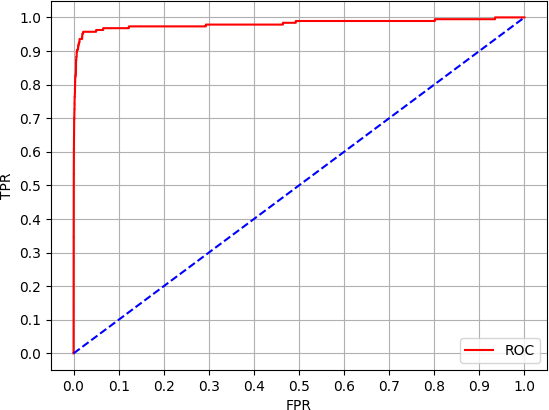
\includegraphics[width=0.44\textwidth]{images/ROC.png}
        \caption{Linear RPN's ROC}
    \end{figure}

    And a graph, showing the decrease of the \emph{true positive ratio} (TPR) and of the \emph{false positive ratio} (FPR) as the threshold increased, as following:

    \begin{figure}[h]
        \centering
        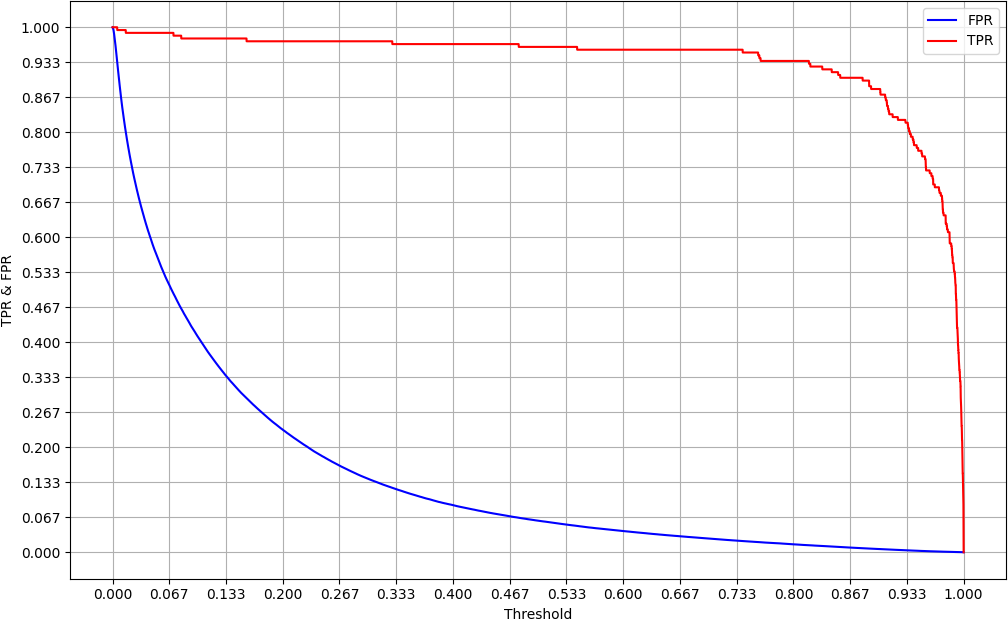
\includegraphics[width=0.44\textwidth]{images/threshold_decision.png}
        \caption{Linear RPN's TPR \& FPR as threshold changes}
    \end{figure}

    From both these graphs we notice our network is indeed able to separate positive and negative anchors with very clear-cut definition. Furthermore, we decided that a good compromise between (TPR) and (FPR) could be achieved by choosing a threshold between $0.8$ and $0.9$: since we didn't want to remove positive anchors too much we put ours at $0.81$. We posit that, to avoid false positives as much as possible, $0.9$ should work fine too.

    \paragraph{Test dataset and stats} After this, in our opinion, fundamental decision was made: we resolved to open Pandora's box and create a test set of around 250 images with multiple mobs in the same shot. Unfortunately, as said previously, we didn't develop our network up to classification of the boxes, and thus a full confusion matrix of those is out of the question. At any rate we show the misclassification table for the anchors (after non-maximum-suppression) scored by our network over the whole test set:

    \begin{table}[htb]
        \centering
        \caption{Misclassification matrix}
        \begin{tabularx}{.3\textwidth}{r|c c}\label{tab:miscl}
            & Label pos. & Label neg. \\
            \hline
            Pred. pos. & 62 & 3545 \\
            Pred. neg. & 17 & 127789
        \end{tabularx}
    \end{table}

    Telling us that, indeed, our threshold works, since the TPR is $0.78$ and the FPR is $0.03$. We would like to point out that, since the labelling of the anchors is itself hyperparameter driven (given the choice of anchors and that of the IoU thresholds used to label them) and that we think to have chosen a combination of these parameters that biases the labels towards the non-object side and, furthermore, given this label by itself already dominates the distribution: it is only normal for the number of positive labels to be so low in the set. If we look at the actual images with the positive region proposals added, we'll appreciate much more positive-looking (that may not actually be labelled as positive) proposals than the anchor labelling would actually suggest.

    \paragraph{Going fully convolutional} As said above, we also tried fitting a fully convolutional version of the RPN, unfortunately though the results were pretty mediocre, its ROC pretty clearly showing it:

    \begin{figure}[h]
        \centering
        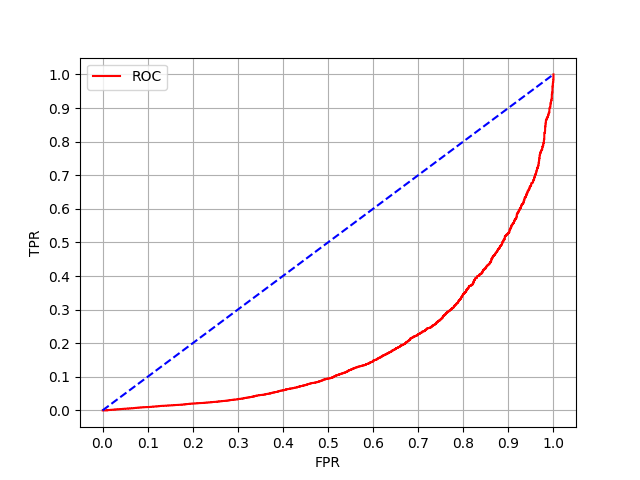
\includegraphics[width=0.44\textwidth]{images/ROC_conv.png}
        \caption{Fully convolutional RPN's ROC}
    \end{figure}

    Indeed this version is unable to sufficiently separate positive and negative samples, leading to unacceptable predictions\dots a shame, since it would've been several magnitudes lighter (weighing just $3.5$ mbs) and faster (both to execute and to train) than its linear counterpart.
    \newpage
    \paragraph{Looking at results} Let's now give a look at some proposals formulated by our network:

    \begin{figure}[h]
        \centering
        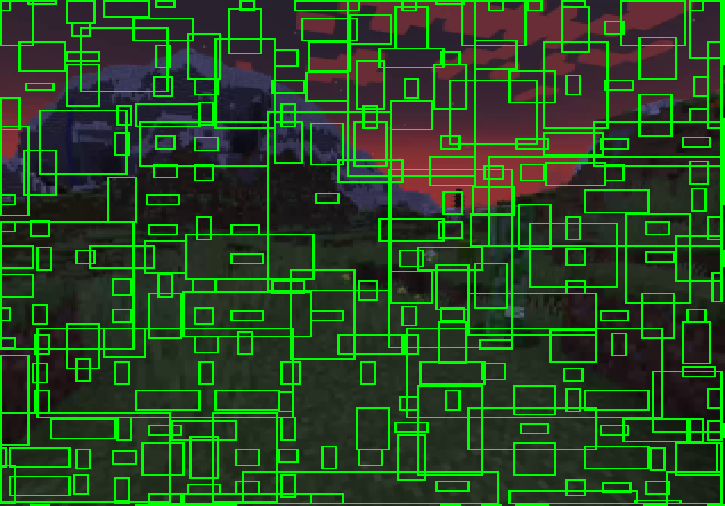
\includegraphics[width=0.44\textwidth]{images/sunset.png}
        \caption{An \emph{interesting} sunset}
    \end{figure}

    Before looking at the good stuff, we would like to show the bad/interesting stuff.  TODO, Dario.

    \begin{figure}[h]
        \centering
        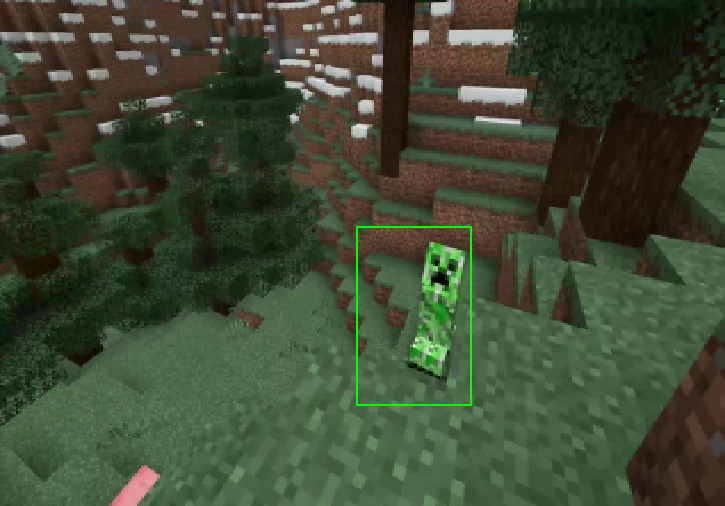
\includegraphics[width=0.44\textwidth]{images/nice_creeper.png}
        \caption{A creeper in his natural habitat}
    \end{figure}

    In this case we can see an excellent result. Alas, one may see there's part of a pig in the bottom-left corner; we don't think that to be an error, to recognize a speck so small and without features would be pretty difficult even for state-of-the-art systems.

    \begin{figure}[h]
        \centering
        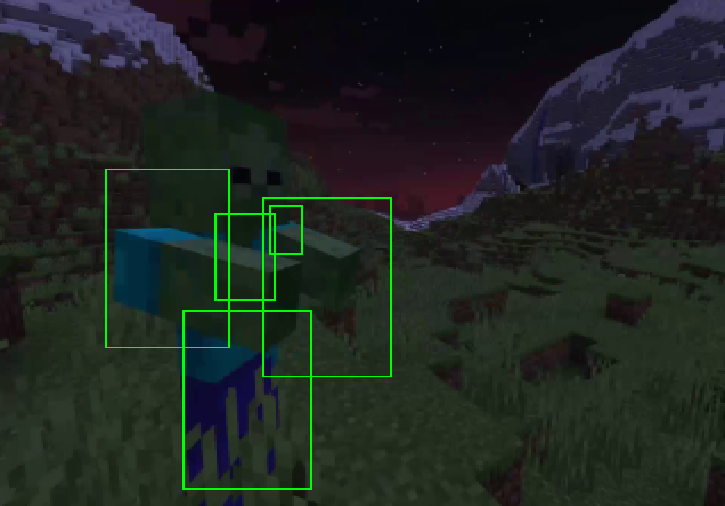
\includegraphics[width=0.44\textwidth]{images/sundered_zombie.png}
        \caption{A zombie, piece-wise}
    \end{figure}

    Here's another good, albeit different, result: in our opinion (and as how the problem is currently formulated, mathematically speaking) a box doesn't have to recognize an object in its entirety,  that's why we accept this sundered recognition as correct. As you may have realized, it is because of this type of proposals that \ref{tab:miscl} holds so many false positives, during the automatic labeling of anchors it is more than possible that the inner anchors of this zombie are classified as negative.

    \begin{figure}[h]
        \centering
        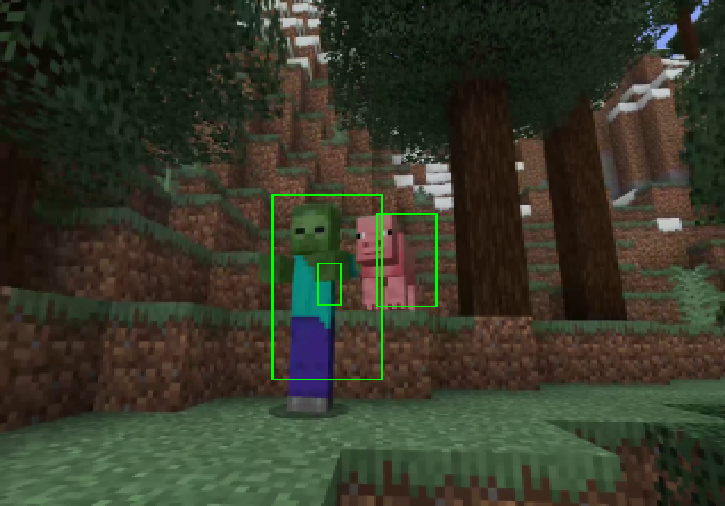
\includegraphics[width=0.44\textwidth]{images/zombie_and_pig.png}
        \caption{Zombie and pig}
    \end{figure}

    In this case we see another sufficiently nice result\dots let's end with two other interesting proposals.

    \begin{figure}[h]
        \centering
        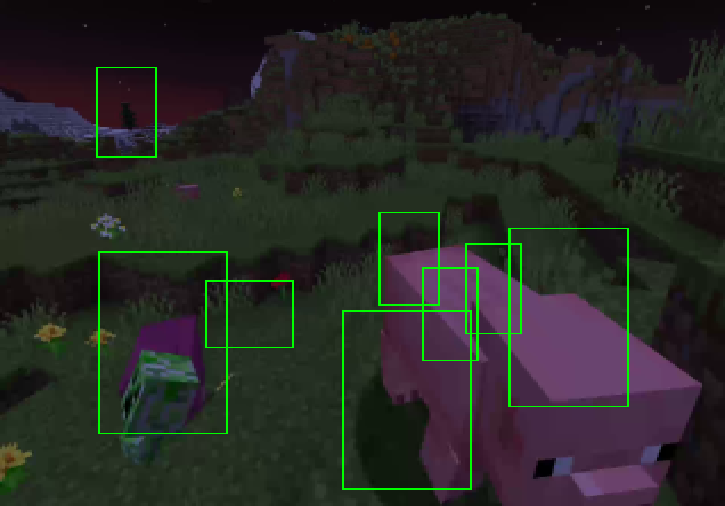
\includegraphics[width=0.44\textwidth]{images/pine.png}
        \caption{Pareidolia in the background}
    \end{figure}

    Leaving the interesting proposals for the pig, the creeper and the sheep in the image, we can see a pine in the upper left corner which has been spot-on proposed by our network: we can't say for certain, but we assume this to be a case of misclassification given by pareidolia, after all to a fast glance that may \emph{seem} like a zombie.

    \newpage
    \begin{figure}[h]
        \centering
        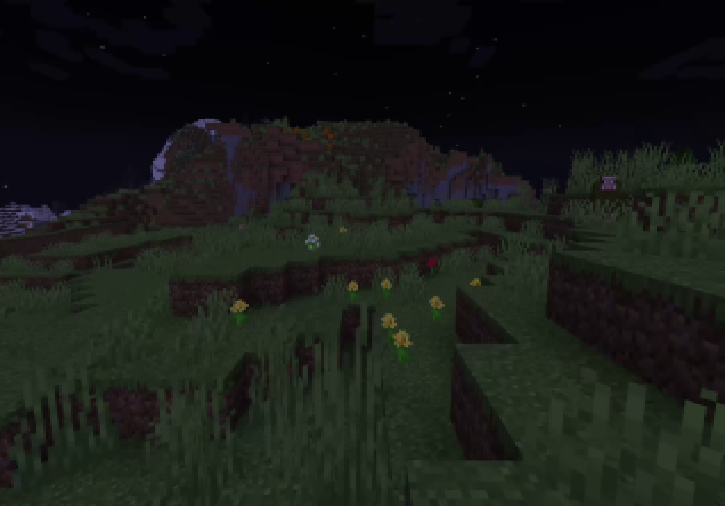
\includegraphics[width=0.44\textwidth]{images/spot_sheep.png}
        \caption{Spot the sheep}
    \end{figure}

    The network gave no proposals for this image, but unfortunately there \emph{is} a sheep in there; but it is probably too green and not in the foreground to be detected.

    In light of these agreeable and interesting results, we think to have reached our goals, not without hiccups nor errors that is. But the network seems to be, generally, well behaved and relatively correct.



    \bibliographystyle{IEEEtran}
    \bibliography{ref}

\end{document}
